% Dieses Dokument muss mit PDFLatex geestzt werden
% Vorteil: Grafiken koennen als jpg, png, ... verwendet werden
%          und die Links im Dokument sind auch gleich richtig
%
\documentclass[
               paper=a4,,
%               twoside, % fuer die Betrachtung am Schirm ungeschickt
% Optionen fuer typearea.
               BCOR1.92mm,DIV12,headinclude, %je hoeher der DIV-Wert, desto mehr geht auf eine Seite - Hack f�r BCOR. Bei BCOR2mm sind die Fuellpunkte beim Inhaltsverzeichnis falsch
%               titlepage,
               bibliography=totoc,
%               idxtotoc,   %Index ins Inhaltsverzeichnis
%				liststotoc, %List of X ins Inhaltsverzeichnis, mit liststotocnumbered werden die Abbildungsverzeichnisse nummeriert
               headsepline,
               cleardoublepage=empty,
               parskip=half,
%				pointlessnumbers, %f"ur englische Texte, dann auch "packages_and_options" und "fonts" anpassen.
%               draft    % um zu sehen, wo noch nachgebessert werden muss - wichtig, da Bindungskorrektur mit drin
               final   % ACHTUNG! - in pagestyle.tex noch Seitenstil anpassen
               ]{scrbook}

%Englisch:			   
%\let\ifdeutsch\iffalse
%\let\ifenglisch\iftrue

%Deutsch:
\let\ifdeutsch\iftrue
\let\ifenglisch\iffalse

			   
%%%
% Beschreibung:
% In dieser Datei werden zuerst die benoetigten Pakete eingebunden und
% danach diverse Optionen gesetzt. Achtung Reihenfolge ist entscheidend!
%
%%%


%%%
% Styleguide:
%
% Ein sehr kleiner Styleguide. Packages werden in Blöcken organisiert.
% Ein Block beginnt mit drei % in einer Zeile, dann % <Blocküberschrift>, dann 
% eine Liste der möglichen Optionen und deren Einstellungen, Gründe und Kommentare
% eine % Zeile in der sonst nichts steht und dann wieder %%% in einer Zeile.
%
% Zwischen zwei Blöcken sind 2 Leerzeilen!
% Zu jedem Paket werden soviele Optionen wie möglich/nötig angegeben
%
%%%

%%%
% Codierung
% Wir sind im 21 Jahrhundert, utf-8 löst so viele Probleme.
%
% Mit UTF-8 funktionieren folgende Pakete nicht mehr. Bitte beachten!
%   * fancyvrb mit § 
%   * easylist -> http://www.ctan.org/tex-archive/macros/latex/contrib/easylist/ 
\usepackage[utf8]{inputenc}
%
%%%

%%%
%Parallelbetrieb tex4ht und pdflatex
\makeatletter
\@ifpackageloaded{tex4ht}{\def\iftex4ht{\iftrue}}
                         {\def\iftex4ht{\iffalse}}
\makeatother
%%%


%%%
%Farbdefinitionen
\usepackage[hyperref,dvipsnames]{xcolor}
%


%%%
% Neue deutsche Rechtschreibung und Literatur statt "Literature", Nachfolger von ngerman.sty
\ifdeutsch
\usepackage[ngerman]{babel}
  %Ein "abstract" ist eine "Kurzfassung", keine "Zusammenfassung"
  \addto\captionsngerman{%
    \renewcommand\abstractname{Kurzfassung}%
  }
\else
%
%
% if you are writing in english
% für englische Texte, Hinweise zu weiteren, notwendigen Umstellungen in README.txt beachten
\usepackage[american]{babel}
\fi
%
%%%

%%%
% Anführungszeichen
% Zitate in \enquote{...} setzen, dann werden automatisch die richtigen Anführungszeichen verwendet.
\usepackage{csquotes}
%%%


%%%
% erweitertes Enumerate
\usepackage{paralist}
%
%%%


%%%
% fancyheadings (nicht nur) fuer koma
\usepackage[automark]{scrpage2} 
%
%%%


%%%
%Mathematik
%
\usepackage[fleqn,leqno]{amsmath} % Viele Mathematik-Sachen: Doku: /usr/share/doc/texmf/latex/amsmath/amsldoc.dvi.gz
%fleqn (=Gleichungen linksbündig platzieren) funktioniert nicht direkt. Es muss noch ein Patch gemacht werden:
\addtolength\mathindent{1em}%work-around ams-math problem with align and 9 -> 10
\usepackage{mathtools} %fixes bugs in AMS math
%
%for theorems, replacement for amsthm
\usepackage[amsmath,hyperref]{ntheorem}
\theorempreskipamount 2ex plus1ex minus0.5ex
\theorempostskipamount 2ex plus1ex minus0.5ex
\theoremstyle{break}
\newtheorem{definition}{Definition}[section]
%
%%%


%%%
% Intelligentes Leerzeichen um hinter Abkürzungen die richtigen Abstände zu erhalten, auch leere.
% siehe commands.tex \gq{}
\usepackage{xspace}
%
%%%


%%%
% Anhang
\usepackage{appendix}
%[toc,page,title,header]
%
%%%


%%%
% Grafikeinbindungen
\usepackage{graphicx}%Parameter "pdftex" unnoetig
\graphicspath{{\getgraphicspath}}
\newcommand{\getgraphicspath}{graphics/}
%
%%%


%%%
% Enables inclusion of SVG graphics - 1:1 approach
% This is NOT the approach of http://www.ctan.org/tex-archive/info/svg-inkscape,
% which allows text in SVG to be typeset using LaTeX
% We just include the SVG as is
\usepackage{epstopdf}
\epstopdfDeclareGraphicsRule{.svg}{pdf}{.pdf}{%
  inkscape -z -D --file=#1 --export-pdf=\OutputFile
}
%
%%%


%%%
% Enables inclusion of SVG graphics - text-rendered-with-LaTeX-approach
% This is the approach of http://www.ctan.org/tex-archive/info/svg-inkscape,
\newcommand{\executeiffilenewer}[3]{%
\IfFileExists{#2}
{
%\message{file #2 exists}
\ifnum\pdfstrcmp{\pdffilemoddate{#1}}%
{\pdffilemoddate{#2}}>0%
{\immediate\write18{#3}}
\else
{%\message{file up to date #2}
}
\fi%
}{
%\message{file #2 doesn't exist}
%\message{argument: #3}
%\immediate\write18{echo "test" > xoutput.txt}
\immediate\write18{#3}
}
}
\newcommand{\includesvg}[1]{%
\executeiffilenewer{#1.svg}{#1.pdf}%
{
inkscape -z -D --file=\getgraphicspath#1.svg %
--export-pdf=\getgraphicspath#1.pdf --export-latex}%
\input{\getgraphicspath#1.pdf_tex}%
}
%%%

%%%
% Tabellenerweiterungen
\usepackage{array} %increases tex's buffer size and enables ``>'' in tablespecs
\usepackage{longtable}
%
%%%

%%%
% Eine Zelle, die sich über mehrere Zeilen erstreckt.
% Siehe Beispieltabelle in Kapitel 2
\usepackage{multirow}
%
%%%


%%%
% Links verhalten sich so, wie sie sollen
\usepackage{url}
%
%%%


%%%
% Index über Begriffe, Abkürzungen
%\usepackage{makeidx} makeidx ist out -> http://xindy.sf.net verwenden
%
%%%

%%%
%lustiger Hack fuer das Abkuerzungsverzeichnis
%nach latex durchlauf folgendes ausfuehren
%makeindex ausarbeitung.nlo -s nomencl.ist -o ausarbeitung.nls 
%danach nochmal latex
%\usepackage{nomencl}
%	\let\abk\nomenclature %Deutsche Ueberschrift setzen
%	  	\renewcommand{\nomname}{List of Abbreviations}
%		%Punkte zw. Abkuerzung und Erklaerung
%	  	\setlength{\nomlabelwidth}{.2\hsize}
%	  	\renewcommand{\nomlabel}[1]{#1 \dotfill}
%		%Zeilenabstaende verkleinern
%	  	\setlength{\nomitemsep}{-\parsep}
%	\makenomenclature
%
%%%

%%%
% Logik für Tex
\usepackage{ifthen} %fuer if-then-else @ commands.tex
%
%%%


%%%
% unterschiedliche Fancy-Chapter-Styles
%\usepackage[Bjarne]{fncychap}
%\usepackage[Lenny]{fncychap}
%
%%%


%%%
%
\usepackage{listings}
%
%%%


%%%
%Alternative zu Listings ist fancyvrb. Kann auch beides gleichzeitig benutzt werden.
\usepackage{fancyvrb}
%\fvset{fontsize=\small} %Groesse fuer den Fliesstext. Falls deaktiviert: \normalsize
%Funktioniert mit UTF-8 nicht mehr
%\DefineShortVerb{\§} %Somit kann im Text ganz einfach |verbatim| text gesetzt werden.
\RecustomVerbatimEnvironment{Verbatim}{Verbatim}{fontsize=\footnotesize}
\RecustomVerbatimCommand{\VerbatimInput}{VerbatimInput}{fontsize=\footnotesize}
%
%%%


%%%
% Bildunterschriften bei floats genauso formatieren wie bei Listings
% Anpassung wird unten bei den newfloat-Deklarationen vorgenommen
% Caption2 vielleicht besser
\usepackage{caption}
%
%%%


%%%
% Ermoeglicht es, Abbildungen um 90 Grad zu drehen
% Alternatives Paket: rotating Allerdings wird hier nur das Bild gedreht, während bei lscape auch die PDF-Seite gedreht wird. 
%Das Paket lscape dreht die Seite auch nicht 
\usepackage{pdflscape}
%
%%%


%%%
% Fuer listings
% Wird für fancyvrb und für lstlistings verwendet
% zustäzlich für den Paramter [H] = Floats WIRKLICH da wo sie deklariert wurden paltzieren - ganz ohne Kompromisse
% floatrow ist der Nachfolger von float
\iftex4ht
\usepackage{float}
\else
%tex4ht is not compatible with the advanced floatrow package
\usepackage{floatrow}
\fi
%
%%%


%%%
% Fuer Abbildungen innerhalb von Abbildungen
% Ersetzt das Paket subfigure
%\usepackage{subfig}
%
%%%


%%%
%Fuer Tabellen mit Variablen Spaltenbreiten
%\usepackage{tabularx}
%\usepackage{tabulary}
%
%%%


%%%
% Fußnoten
% 
%\usepackage{dblfnote}  %Zweispaltige Fußnoten
%
% Keine hochgestellten Ziffern in der Fußnote (KOMA-Script-spezifisch):
%\deffootnote[1.5em]{0pt}{1em}{\makebox[1.5em][l]{\bfseries\thefootnotemark}} 
%
% Abstand zwischen Fußnoten vergrößern:
%\setlength{\footnotesep}{.85\baselineskip}
%
%
\renewcommand{\footnoterule}{}             % Keine Trennlinie zur Fußnote 
\addtolength{\skip\footins}{\baselineskip} % Abstand Text <-> Fußnote
% Fußnoten immer ganz unten auf einer \raggedbottom-Seite
\usepackage{fnpos}
%
%%%


%%%
%
\raggedbottom     % Variable Seitenhöhen zulassen
%
%%%


%%%
% Falls die Seitenzahl bei einer Referenz auf eine Abbildung nur dann angegeben werden soll,
% falls sich die Abbildung nicht auf der selben Seite befindet...
\iftex4ht
%tex4ht does not work well with vref, therefore we emulate vref behavior
\newcommand{\vref}[1]{\ref{#1}}
\else
\ifdeutsch
\usepackage[ngerman]{varioref}
\else
\usepackage{varioref}
\fi
\fi
%%%

%%%
% Noch schoenere Tabellen als mit booktabs mit http://www.zvisionwelt.de/downloads.html
\usepackage{booktabs} 
%
%\usepackage[section]{placeins}
%
%%%


%%%
%Fuer Graphiken. Allerdings funktioniert es nicht zusammen mit pdflatex
%\usepackage{gastex} % \tolarance kann dann nicht mehr umdefiniert werden
%
%%%


%%%
%
%\usepackage{multicol}
%\usepackage{setspace} % kollidiert mit diplomarbeit.sty
%
%http://www.tex.ac.uk/cgi-bin/texfaq2html?label=floats
%\usepackage{flafter} %floats IMMER nach ihrer Deklaration platzieren
%
%%%


%%%
%schoene TODOs
\usepackage{todonotes}
\let\xtodo\todo
\renewcommand{\todo}[1]{\xtodo[inline,color=black!5]{#1}}
\newcommand{\utodo}[1]{\xtodo[inline,color=green!5]{#1}}
\newcommand{\itodo}[1]{\xtodo[inline]{#1}}
%
%%%


%%%
% Neue Pakete bitte VOR hyperref einbinden. Insbesondere bei Verwendung des
% Pakets "index" wichtig, da sonst die Referenzierung nicht funktioniert.
% Für die Indizierung selbst ist unter http://xindy.sourceforge.net
% ein gutes Tool zu erhalten 
%%%


%%%
%
% hier also neue packages einbinden
%
%%%


%%%
% ggf.in der Endversion komplett rausnehmen. dann auch \href in commands.tex aktivieren
% Alle Optionen nach \hypersetup verschoben, sonst crash
%
\usepackage[]{hyperref}%siehe auch: "Praktisches LaTeX" - www.itp.uni-hannover.de/~kreutzm
%
%% Da es mit KOMA 3 und xcolor zu Problemen mit den global Options kommt MÜSSEN die Optionen so gesetzt werden.
%

% Eigene Farbdefinitionen ohne die Namen des xcolor packages
\definecolor{darkblue}{rgb}{0,0,.5}
\definecolor{black}{rgb}{0,0,0}

\hypersetup{
	breaklinks=true,
	bookmarksnumbered=true,
	bookmarksopen=true,
	bookmarksopenlevel=1,
	breaklinks=true,
	colorlinks=true,
	pdfstartview=Fit,
	pdfpagelayout=SinglePage,
	%
	filecolor=darkblue,
	urlcolor=darkblue,
	linkcolor=black,
	citecolor=black
}
%
%%%


%%%
% cleveref für cref statt autoref, da cleveref auch bei Definitionen funktioniert
\ifdeutsch
\usepackage[ngerman,capitalise,nameinlink]{cleveref}
\else
\usepackage[capitalise,nameinlink]{cleveref}
\fi
%%%


%%%
% Zur Darstellung von Algorithmen
% Algorithm muss nach hyperref geladen werden
\usepackage[chapter]{algorithm} 
\usepackage[]{algpseudocode}
%
%%%


%%%
% Schriften
%%%
%
\automark[section]{chapter}
\setkomafont{pageheadfoot}{\normalfont\sffamily}
\setkomafont{pagenumber}{\normalfont\rmfamily}
%\setheadsepline[.4pt]{.4pt} %funktioniert nicht: Alle Linien sind hier weg
%
%%%

%%%
%
\ifenglisch
% Fuer englische Texte sind serifenhafte Ueberschriften gut. Deshalb hier der Befehl zum Aktivieren von serifenhaften Ueberschriften
\setkomafont{disposition}{\normalfont\rmfamily}

% Bei englisschen Texten das Label (optionaler Eintrag bei \item) bei description-Umgegungen nur auf fett und nicht fett+serifenlos stellen.
\setkomafont{descriptionlabel}{\normalfont\bfseries}
\fi
%
%%%

%%%
% Fuer deutsche Texte: Weniger Silbentrennung, mehr Abstand zwischen den Woertern
\ifdeutsch
\setlength{\emergencystretch}{3em} % Silbentrennung reduzieren durch mehr frei Raum zwischen den Worten
\fi
%%%

%Symbole
%--------
%\usepackage[geometry]{ifsym} % \BigSquare
%\usepackage{mathabx}
%\usepackage{stmaryrd} %fuer \ovee, \owedge, \otimes
%\usepackage{marvosym} %fuer \Writinghand %patched to not redefine \Rightarrow
%\usepackage{mathrsfs} %mittels \mathscr{} schoenen geschwungenen Buchstaben erzeugen
%\usepackage{calrsfs} %\mathcal{} ein bisserl dickeren buchstaben erzeugen - sieht net so gut aus.
                      %durch mathpazo ist das schon definiert
\usepackage{amssymb}

%name-clashes von marvosym und mathabx vermeiden:
\def\delsym#1{%
%  \expandafter\let\expandafter\origsym\expandafter=\csname#1\endcsname
%  \expandafter\let\csname orig#1\endcsname=\origsym
  \expandafter\let\csname#1\endcsname=\relax
}

%\usepackage{pifont}
%\usepackage{bbding}
%\delsym{Asterisk}
%\delsym{Sun}\delsym{Mercury}\delsym{Venus}\delsym{Earth}\delsym{Mars}
%\delsym{Jupiter}\delsym{Saturn}\delsym{Uranus}\delsym{Neptune}
%\delsym{Pluto}\delsym{Aries}\delsym{Taurus}\delsym{Gemini}
%\delsym{Rightarrow}
%\usepackage{mathabx} - Ueberschreibt leider zu viel - und die \le-Zeichen usw. sehen nicht gut aus!


%Fallback-Schriftart
%\usepackage{lmodern}  % Latin Modern Fonts sind die Nachfolger von Computer Modern, den LaTeX-Standardfonts
%Quelle: http://homepage.ruhr-uni-bochum.de/Georg.Verweyen/pakete.html
%Allerdings sieht diese Schritart in Diplomarbeiten fuer Fliesstext auch nicht besonders schoen aus.
%Trotzdem ist sie fuer Programmcode gut geeignet

%Schriftart fuer die Ueberschriften - ueberschreibt lmodern
\ifdeutsch
\usepackage[scaled=.95]{helvet}
\else
\usepackage[scaled=.90]{helvet}
\fi

%Schriftart fuer Programmcode - ueberschreibt lmodern
%Falls auskommentiert, wird die Standardschriftart genommen
%\usepackage[scaled=.92]{luximono} % Fuer schreibmaschinenartige Schluesselwoerter in den Listings - geht bei alten Installationen nicht, da einige Fontshapes (<>=) fehlen
%\usepackage{courier} 

% Tolle Schriften...
%\usepackage{helvet}
%\usepackage{palatino}
%\usepackage[osf]{libertine}
% Für Schreibschrift würde tun, muss aber ned
%\usepackage{mathrsfs} %  \mathscr{ABC}


%Schriftart fuer den Fliesstext - ueberschreibt lmodern
%
\ifdeutsch
\usepackage[osf]{mathpazo} %ftp://ftp.dante.de/tex-archive/fonts/mathpazo/ - Tipp aus DE-TEX-FAQ 8.2.1
\fi
%Bringt Palantino, osf = Minuskel-Ziffern
%
%\usepackage{charter} %Charter fuer englsiche Texte
%\linespread{1.05} % Durchschuss für Charter leicht erhöhen
%
%\usepackage{mathptmx} %Times fuer englische Texte. Sieht nicht sooo gut aus.
\ifenglisch
\usepackage{lmodern}
\fi

\usepackage[T1]{fontenc}


% optischer Randausgleich - bei miktex gleich dabei - bei linux von
%  http://www.ctan.org/tex-archive/macros/latex/contrib/microtype/
%  herunterladen 
\usepackage{microtype}
%Falls bei einer Silbentrennung ploetzlich eine ganze Zeile fehlt (passiert unter Windows XP mit MikTex 2.5 und foxit reader als pdfreader
%\usepackage{pdfcprot}
%ausprobieren. Dieses erzeugt allerdings nur für Palatino (in dieser Vorlage die Default-Schrift) einen guten optischen Randausgleich
%Falls alle Stricke reissen, muss leider auf den optischen Randausgleich verzichtet werden.

%fuer microtype
%tracking=true muss als Parameter des microtype-packages mitgegeben werden
%
%Deaktiviert, da dies bei Algorithmen seltsam aussieht
%
%\DeclareMicrotypeSet*[tracking]{my}{ font = */*/*/sc/* }% 
%\SetTracking{ encoding = *, shape = sc }{ 45 }% Hier wird festgelegt,
            % dass alle Passagen in Kapitälchen automatisch leicht
            % gesperrt werden.
			% Quelle: http://homepage.ruhr-uni-bochum.de/Georg.Verweyen/pakete.html

%
%%%


%%%
% Links auf Gleitumgebungen springen nicht zur Beschriftung,
% Doc: http://mirror.ctan.org/tex-archive/macros/latex/contrib/oberdiek/hypcap.pdf
% sondern zum Anfang der Gleitumgebung
\usepackage[all]{hypcap}
%%%


%%%
% Deckblattstyle
%
% für englische Ausarbeitungen "language=english" benutzen
\usepackage[
	title={Förderungswürdigkeit der F\"{o}rderung von Öl},
	author={Lars K.},
	type=bachelor,
	institute=iaas,
	number=12345,
	course=se,
	examiner={Prof.\ Dr.\ Uwe Fessor},
	supervisor={Dipl.-Inf.\ Roman Tiker,\\Dipl.-Inf.\ Laura Stern},
	startdate={5.\ Juli 2013}, % English: July 5, 2013;    ISO: 2013-07-05
	enddate={5.\ Januar 2014}, % English: January 5, 2014; ISO: 2014-01-05
	crk={I.7.2},
	language=german
	%language=english
	]{uni-stuttgart-cs-cover/uni-stuttgart-cs-cover}
%
%%%


%%%
%Bugfixes packages
\usepackage{fixltx2e} %Bereinigt einige Ungereimtheiten, die auf Grund von Rueckwaertskompatibilitaet beibahlten wurden.
%\usepackage{mparhack} %Fixt die Position von marginpars (die in DAs selten bis gar nicht gebraucht werden}
%\usepackage{ellipsis} %Fixt die Abstaende vor \ldots. Wird wohl auch nicht benoetigt.
%
%%%


%%%
% Rand
%Viele Moeglichkeiten, die Raender im Dokument einzustellen.
%Satzspiegel neu berechnen. Dokumentation dazu ist in "scrguide.pdf" von KOMA-Skript zu finden
%  Optionen werden bei \documentclass[] in ausarbeitung.tex mitgegeben.
\typearea[current]{current} %neu berechnen, da neue Schrift eingebunden

%\usepackage{a4}
%\usepackage{a4wide}
%\areaset{170mm}{277mm} %a4:29,7hochx21mbreit

%Wer die Masse direkt eingeben moechte:
%Bei diesem Beispiel wird die Regel nicht beachtet, dass der innere Rand halb so gross wie der aussere Rand und der obere Rand halb so gross wie der untere Rand sein sollte
%\usepackage[inner=2.5cm, outer=2.5cm, includefoot, top=3cm, bottom=1.5cm]{geometry}



%
%%%


%%%
% Optionen                                                                  
%
%Skip=0 funktioniert nicht
\captionsetup{format=hang,labelfont=bf,justification=justified,singlelinecheck=false,skip=0pt}
%
%neue float Umgebung fuer Listings, die mittels fancyvrb gesetzt werden sollen
\floatstyle{ruled}
\newfloat{Listing}{tbp}{code}[chapter]
\newfloat{Algorithmus}{tbp}{alg}[chapter]
%
%amsmath
%\numberwithin{equation}{section}
%\renewcommand{\theequation}{\thesection.\Roman{equation}}
%
%pdftex
\pdfcompresslevel=9
%
%Tabellen (array.sty)
\setlength{\extrarowheight}{1pt}
%
%

% Andere Kapitelueberschriften
% falls einem der Standard von KOMA nicht gefaellt...
% Falls man zurück zu KOMA moechte, dann muss jede der vier folgenden Moeglichkeiten deaktiviert sein.

% 1. Moeglichkeit
%\usepackage[Sonny]{fncychap}

% 2. Moeglichkeit
\iffalse
\usepackage[Bjarne]{fncychap}
\ChNameVar{\Large\sf} \ChNumVar{\Huge} \ChTitleVar{\Large\sf}
\ChRuleWidth{0.5pt} \ChNameUpperCase
\fi

%Variante der 2. Moeglichkeit
\iffalse
\usepackage[Rejne]{fncychap}
\ChNameVar{\centering\Huge\rm\bfseries}
\ChNumVar{\Huge}
 \ChTitleVar{\centering\Huge\rm}
\ChNameUpperCase
\ChTitleUpperCase
\ChRuleWidth{1pt}
\fi

% 3. Moeglichkeit
\iffalse
\usepackage{fncychap}
\ChNameUpperCase
\ChTitleUpperCase
\ChNameVar{\raggedright\normalsize} %\rm
\ChNumVar{\bfseries\Large}
\ChTitleVar{\raggedright\Huge}
\ChRuleWidth{1pt}
\fi

% 4. Moeglichkeit
% Zur Aktivierierung "\iffalse" und "\fi" auskommentieren
% Innen drin kann man dann noch zwischen
%   * serifenloser Schriftart (eingestellt)
%   * serifenhafter Schriftart (wenn kein zusaetzliches Kommando aktiviert ist) und
%   * Kapitälchen wählen
\iffalse
\makeatletter
%\def\thickhrulefill{\leavevmode \leaders \hrule height 1ex \hfill \kern \z@}

%Fuer Kapitel mit Kapitelnummer
\def\@makechapterhead#1{%
  \vspace*{10\p@}%
  {\parindent \z@ \raggedright \reset@font
			%Default-Schrift: Serifenhaft (gut fuer englische Dokumente)
            %A) Fuer serifenlose Schrift:
            \fontfamily{phv}\selectfont
			%B) Fuer Kapitaelchen:
			%\fontseries{m}\fontshape{sc}\selectfont
            %C) Fuer ganz "normale" Schrift:
            %\normalfont 
			%
			\Large \@chapapp{} \thechapter
        \par\nobreak\vspace*{10\p@}%
        \interlinepenalty\@M
    {\Huge\bfseries\baselineskip3ex
	%Fuer Kapitaelchen folgende Zeile aktivieren:
	%\fontseries{m}\fontshape{sc}\selectfont
	#1\par\nobreak}
    \vspace*{10\p@}%
\makebox[\textwidth]{\hrulefill}%    \hrulefill alone does not work
    \par\nobreak
    \vskip 40\p@
  }}

  %Fuer Kapitel ohne Kapitelnummer (z.B. Inhaltsverzeichnis)
  \def\@makeschapterhead#1{%
  \vspace*{10\p@}%
  {\parindent \z@ \raggedright \reset@font
            \normalfont \vphantom{\@chapapp{} \thechapter}
        \par\nobreak\vspace*{10\p@}%
        \interlinepenalty\@M
    {\Huge \bfseries %
	%Default-Schrift: Serifenhaft (gut fuer englische Dokumente)
    %A) Fuer serifenlose Schrift folgende Zeile aktivieren:
    \fontfamily{phv}\selectfont
	%B) Fuer Kapitaelchen folgende Zeile aktivieren:
	%\fontseries{m}\fontshape{sc}\selectfont
	#1\par\nobreak}
    \vspace*{10\p@}%
\makebox[\textwidth]{\hrulefill}%    \hrulefill does not work
    \par\nobreak
    \vskip 40\p@
  }}
%
\makeatother
\fi

%
%%%


%%%
%Minitoc-Einstellungen
%\dominitoc
%\renewcommand{\mtctitle}{Inhaltsverzeichnis dieses Kapitels}
%
% Disable single lines at the start of a paragraph (Schusterjungen)
\clubpenalty = 10000
%
% Disable single lines at the end of a paragraph (Hurenkinder)
\widowpenalty = 10000 \displaywidowpenalty = 10000
%
%http://groups.google.de/group/de.comp.text.tex/browse_thread/thread/f97da71d90442816/f5da290593fd647e?lnk=st&q=tolerance+emergencystretch&rnum=5&hl=de#f5da290593fd647e
%Mehr Infos unter http://www.tex.ac.uk/cgi-bin/texfaq2html?label=overfull
\tolerance=2000
\setlength{\emergencystretch}{3pt}   % kann man evtl. auf 20 erhoehen
\setlength{\hfuzz}{1pt}
%
%%%


%%%
% Fuer listings.sty
\lstset{language=XML,
        showstringspaces=false,
        extendedchars=true,
        basicstyle=\footnotesize\ttfamily,
        commentstyle=\slshape,
        stringstyle=\ttfamily, %Original: \rmfamily, damit werden die Strings im Quellcode hervorgehoben		zusaetzlich evtl.: \scshape oder \rmfamily durch \ttfamily ersetzen. Dann sieht's aus, wie bei fancyvrb
        breaklines=true,
        breakatwhitespace=true,
        columns=flexible,
        aboveskip=0mm, %deaktivieren, falls man lstlistings direkt als floating object benutzt (\begin{lstlisting}[float,...])
        belowskip=0mm, %deaktivieren, falls man lstlistings direkt als floating object benutzt (\begin{lstlisting}[float,...])
        captionpos=b
}
\ifdeutsch
\renewcommand{\lstlistlistingname}{Verzeichnis der Listings}
\fi
%
%%%


%%%
%fuer algorithm.sty: - falls Deutsch und nicht Englisch. Falls Englisch als Sprache gewählt wurde, bitte die folgenden beiden Zeilen auskommentieren.
\floatname{algorithm}{Algorithmus}
\ifdeutsch
\renewcommand{\listalgorithmname}{Verzeichnis der Algorithmen}
\fi
%
%%%


%%%
% Das Euro Zeichen 
% Fuer Palatino (mathpazo.sty): richtiges Euro-Zeichen
% Alternative: \usepackage{eurosym}
\newcommand{\EUR}{\ppleuro}
%
%%%


%%%
%
% Float-placements - http://dcwww.camd.dtu.dk/~schiotz/comp/LatexTips/LatexTips.html#figplacement
% and http://people.cs.uu.nl/piet/floats/node1.html
\renewcommand{\topfraction}{0.85}
\renewcommand{\bottomfraction}{0.95}
\renewcommand{\textfraction}{0.1}
\renewcommand{\floatpagefraction}{0.75}
%\setcounter{totalnumber}{5}
%
%%%

%%%
%
% Bei Gleichungen nur dann die Nummer zeigen, wenn die Gleichung auch referenziert wird
%
% Funktioniert mit MiKTeX Stand 2012-01-13 nicht. Deshalb ist dieser Schalter deaktiviert.
%
%\mathtoolsset{showonlyrefs}
%
%%%

%%%
%Optischer Randausgleich
\usepackage{microtype}
%%%

%%%
% Rueckverweise aus dem Literaturverzeichnis
\usepackage[hyperpageref]{backref}
\ifdeutsch
% Deutscher Text
\newcommand{\babelbackrefnotcited}{\relax}
\newcommand{\babelbackrefcitedsingle}[1]{(Zitiert auf Seite~#1)}
\newcommand{\babelbackrefcitedmulti}[1]{(Zitiert auf den Seiten~#1)}
\newcommand{\babelbackrefand}{und}
\else
% Englischer Text
\newcommand{\babelbackrefnotcited}{\relax}
\newcommand{\babelbackrefcitedsingle}[1]{(Cited on page~#1)}
\newcommand{\babelbackrefcitedmulti}[1]{(Cited on pages~#1)}
\newcommand{\babelbackrefand}{and}
\fi
% Tweak backref
\renewcommand{\backreftwosep}{ \babelbackrefand~} % seperate 2 pages
\renewcommand{\backreflastsep}{ \babelbackrefand~} % seperate last of longer list
\renewcommand*{\backref}[1]{} % Standard deaktivieren
\renewcommand*{\backrefalt}[4]{% 
\ifcase #1 %
\babelbackrefnotcited%
\or
\babelbackrefcitedsingle{#2}%
\else
\babelbackrefcitedmulti{#2}%
\fi}
%
%%%




 %Der untere Rand darf "flattern"
\raggedbottom

%%%
% Wie tief wird das Inhaltsverzeichnis aufgeschl�sselt
% 0 --\chapter
% 1 --\section
% 2 --\subsection
% 3 --\subsubsection
% 4 --\paragraph
% fuer kuerzeres Inhaltsverzeichnis verwenden - oder minitoc benutzen
\setcounter{tocdepth}{3}
%
%%%

%Sprache f"ur das Titelblatt einstellen. Standard: deutsch
\ifenglisch
\sprache{englisch}
\fi

\makeindex

\pruefer{Prof.\,Dr.\,Pro Fessor}
\betreuer{Dipl.-Inf.\,Roman Tiker} % oder M.\,Sc.\,Roman Tiker

\ifdeutsch
\begonnen{25.\,April 2005}
\beendet{21.\,Oktober 2005}
\else
%Bei englischen Arbeiten ist das Format "October 21, 2005" (siehe http://www.ego4u.de/de/cram-up/vocabulary/date/written)
\begonnen{April 25, 2005}
\beendet{Oktober 21, 2005}
\fi

\titel{Web Services und empirische Philosophie}
\autor{Au Torin}
%\autor{C.\,O.\,Autor}  % bei zwei Autoren
%\studiengang{swt} % Default ist \studiengang{inf}, also Informatik.

\nummer{4712}

%Hier das Institut angeben.
%\institut\fmi
%\institut\iris
%\institut\iste
%\institut\iti
%\institut\iaas
%\institut\ipvs
%\institut\vis
%\institut\visus

%Alternativen:

%1. Freitext
\institut{
Institut f\"ur Formale Methoden der Informatik\\\vskip .3em
Abteilung Formale Konzepte\\\vskip .3em
Universit\"at Stuttgart\\
Universit\"atsstra{\ss}e 38\\
D--70569 Stuttgart}

%2. Ganze Fakultaet
%\institut\fak


%Bitte CR-Klassifikationen anpassen
%  http://www.informatik.uni-stuttgart.de/zdi/buecherei/ifibib_hilfe_cr.html 
%  oder
%  http://www.acm.org/class/
\crk{H.4.1}%Office Automation: Workflow Management
\crk{K.1} %Computer Industry: standards

%Angaben in die PDF-Infos uebernehmen
\makeatletter
\hypersetup{
            pdftitle={\@titel},
            pdfauthor={\@author},
            pdfkeywords={\@crk}, % <-- hier ggf. weitere Stichworte einfuegen
            pdfsubject={}
}
\makeatother

\begin{document}
%\svnInfo $Id: ausarbeitung.tex 80 2009-04-09 11:06:26Z koppor $ 

%tex4ht-Konvertierung versch�nern
\iftex4ht
% tell tex4ht to create picures also for formulas starting with '$'
% WARNING: a tex4ht run now takes forever!
\Configure{$}{\PicMath}{\EndPicMath}{} 
%$ % <- syntax highlighting fix for emacs
\Css{body {text-align:justify;}}

%conversion of .pdf to .png
\Configure{graphics*}  
         {pdf}  
         {\Needs{"convert \csname Gin@base\endcsname.pdf  
                               \csname Gin@base\endcsname.png"}%  
          \Picture[pict]{\csname Gin@base\endcsname.png}%  
         }  
\fi

\VerbatimFootnotes %verbatim text in Fussnoten erlauben. Geht normalerweise nicht.
%\frontmatter
% $Id: commands.tex 80 2009-04-09 11:06:26Z koppor $
%
%wird fuer Tabellen benoetigt (z.B. >{centering\RBS}p{2.5cm} erzeugt einen zentrierten 2,5cm breiten Absatz in einer Tabelle
\newcommand{\RBS}{\let\\=\tabularnewline}

%Normalerweise werden Texte mittels ``Satz'' beschrieben.
%Dann werden auch die richtigen Anfuehrungszeichen verwendet.
%Manchmal klappt es doch nicht. Und statt \glqq Test\grqq{} ... wird
%hier das Kommando \gq definiert, dass sich \gq{so} benutzt.
% siehe reader für richtige variante
\newcommand{\gq}[1]{\glqq{}#1\grqq{}\xspace}

%% typoraphisch richtige Abkürzungen
\newcommand{\zB}[0]{z.\,B.\xspace}
\newcommand{\bzw}[0]{bzw. \xspace}

%from hmks makros.tex - \indexify
\newcommand{\toindex}[1]{\index{#1}#1}
%
\newcommand{\dotcup}{\ensuremath{\,\mathaccent\cdot\cup\,}} %Tipp aus The Comprehensive LaTeX Symbol List
%
%Anstatt $|x|$ $\abs{x}$ verwenden. Die Betragsstriche skalieren automatisch, falls "x" etwas groessers sein sollte...
\newcommand{\abs}[1]{\left\lvert#1\right\rvert}
%
%fuer Zitate
\newcommand{\citeS}[2]{\cite[S.~#1]{#2}}
\newcommand{\citeSf}[2]{\cite[S.~#1\,f.]{#2}}
\newcommand{\citeSff}[2]{\cite[S.~#1\,ff.]{#2}}
\newcommand{\vgl}{vgl.\ }
\newcommand{\Vgl}{Vgl.\ }
%
\newcommand{\commentchar}{\ensuremath{/\mkern-4mu/}}
\algrenewcommand{\algorithmiccomment}[1]{\hfill $\commentchar$ #1}

% Seitengroessen - Gegen Schusterjungen und Hurenkinder...
\newcommand{\largepage}{\enlargethispage{\baselineskip}}
\newcommand{\shortpage}{\enlargethispage{-\baselineskip}}

\pagenumbering{arabic}
\Titelblatt
%Nach dem Titelblatt ist die aktuelle Seite immer noch 1
%Dies wird mit den naechsten zwei Zeilen korrigiert.
\setcounter{page}{2}
\cleardoublepage

%Jetzt das Inhaltsverzeichnis
%Eigener Seitenstil fuer's Inhaltsverzeichnis
\deftripstyle{preamble}{}{}{}{}{}{\pagemark}
%Doku zu deftripstyle: scrguide.pdf
\pagestyle{preamble}
\renewcommand*{\chapterpagestyle}{preamble}

%Kurzfassung / abstract
%auch im Stil vom Inhaltsverzeichnis
\ifdeutsch
\section*{Kurzfassung}
\else
\section*{Abstract}
\fi
\ldots ... Short summary of the thesis ...
\cleardoublepage

\iftex4ht
\else
\microtypesetup{protrusion=false}
\fi

%%%
% Literaturverzeichnis ins TOC mit aufnehmen, aber nur wenn nichts anderes mehr hilft!
% \addcontentsline{toc}{chapter}{Literaturverzeichnis}
%
% oder zB
%\addcontentsline{toc}{section}{Abk�rzungsverzeichnis}
%\section*{Abk�rzungsverzeichnis}
%
%%%

%Inhaltsverzeichnis anlegen
\tableofcontents

% Bei einem ung�nstigen Seitenumbruch im Inhaltsverzeichnis, kann dieser mit
% \addtocontents{toc}{\protect\newpage}
% an der passenden Stelle im Flie�text erzwungen werden.

%listof* untereinandergesetzt
%ACHTUNG! Falls ein anderer Kapitelstil gew�hlt wird, muss der Code hier evtl.
%  angepasst werden
\begingroup 
\makeatletter
  \def\@makeschapterhead#1{%
  \vspace*{10\p@}%
  {\parindent \z@ \raggedright \reset@font
            \normalfont \vphantom{\@chapapp{} \thechapter}
        \par\nobreak\vspace*{10\p@}%
        \interlinepenalty\@M
    {\huge \bfseries %
	%
	%Default-Schrift: Serifenhaft (fuer englische Dokumente)
	% Dann sowohl A als auch B deaktivieren
    %A) Fuer serifenlose Schrift folgende Zeile aktivieren:
	\ifdeutsch
    \fontfamily{phv}\selectfont
	\fi
	%B) Fuer Kapitaelchen folgende Zeile aktivieren:
	%\fontseries{m}\fontshape{sc}\selectfont
	%
	#1\par\nobreak}
    %\vspace*{1\p@}%
\makebox[\textwidth]{\hrulefill}%    \hrulefill alone does not work
    \par\nobreak
    \vskip 5\p@
  }}
\makeatother
\let\cleardoublepage\clearpage
\listoffigures
\let\cleardoublepage\relax
\listoftables

%Wird nur bei Verwendung von der lstlisting-Umgebung mit dem "caption"-Parameter benoetigt
%\lstlistoflistings 
%ansonsten:
\ifdeutsch
\listof{Listing}{Verzeichnis der Listings}
\else
\listof{Listing}{List of Listings}
\fi

%mittels \newfloat wurde die Algorithmus-Gleitumgebung definiert.
%Mit folgendem Befehl werden alle floats dieses Typs ausgegeben
\ifdeutsch
\listof{Algorithmus}{Verzeichnis der Algorithmen}
\else
\listof{Algorithmus}{List of Algorithms}
\fi
%\listofalgorithms %Ist nur f�r Algorithmen, die mittels \begin{algorithm} umschlossen werden, n�tig

\endgroup

\cleardoublepage

\iftex4ht
\else
%Optischen Randausgleich und Grauwertkorrektur wieder aktivieren
\microtypesetup{protrusion=true}
\fi

\renewcommand*{\chapterpagestyle}{scrplain}
\pagestyle{scrheadings}
% $Id: pagestyle.tex 31 2008-03-16 18:29:38Z koppor $

\pagestyle{scrheadings}

%ihead aufgeteilt - Bezeichnungen: 4.1, S. 119, scrguide

%für die Teilversionen - nur bei Verwendung von RCS/CVS
%\ihead[Version \RCSRevision]{Version \RCSRevision}

%Für die finale Version oder bei Verwendung von SVN
\ihead[]{}


% Sowohl für die Teilversionen als auch die finale Version:

\chead[]{}
\ohead[]{\headmark}
%
\cfoot[]{}
\ofoot[\usekomafont{pagenumber}\thepage]{\usekomafont{pagenumber}\thepage}
\ifoot[]{}

%
%
% ** Hier wird der Text eingebunden **
%
%\svnInfo $Id: einleitung.tex 80 2009-04-09 11:06:26Z koppor $ 

\chapter{Einleitung}
In diesem Kapitel steht die Einleitung zu dieser Diplomarbeit. Sie soll nur als Beispiel dienen und hat nichts mit dem Buch \cite{WSPA} zu tun. Nun viel Erfolg bei der Arbeit!

\section*{Gliederung}
Die Arbeit ist in folgender Weise gegliedert:
\begin{description}
\item[Kapitel~\ref{chap:k2} -- \nameref{chap:k2}:] Hier werden werden die Grundlagen dieser Arbeit beschrieben.
\item[Kapitel~\ref{chap:zusfas} -- \nameref{chap:zusfas}] fasst die Ergebnisse der Arbeit zusammen und stellt Ankn�pfungspunkte vor.
\end{description}

%\input{...weitere Kapitel...}
%\svnInfo $Id: kapitel2.tex 80 2009-04-09 11:06:26Z koppor $ 

%Die Angabe des schlauen Spruchs auf diesem Wege funtioniert nur,
%wenn keine Änderung des Kapitels mittels den in preambel/chapterheads.tex
%vorgeschlagenen Möglichkeiten durchgeführt wurde.
\setchapterpreamble[u]{%
\dictum[Albert Einstein]{Probleme kann man niemals mit derselben Denkweise lösen, durch die sie entstanden sind.}
}
\chapter{Kapitel zwei}
%\vspace{-3cm}
%\vspace{2cm}

\label{chap:k2}
Hier wird der Hauptteil stehen. Falls mehrere Kapitel gewünscht, entweder mehrmals \texttt{\textbackslash{}chapter} benutzen oder pro Kapitel eine eigene Datei anlegen und \texttt{ausarbeitung.tex} anpassen.

Verweise auf einen Abschnitt gehen mittels: ``Siehe Abschnitt~\vref{sec:mf}''. Das Kommando \texttt{\textbackslash{}vref} funktioniert ähnlich wie \texttt{\textbackslash{}ref} mit dem Unterschied, dass zusätzlich ein Verweis auf die Seite hinzugefügt wird. \texttt{vref}: Abschnitt \vref{sec:diff}, \texttt{ref}: \ref{sec:diff}.

Falls ein Abschnitt länger als eine Seite wird und man mittels \texttt{\textbackslash{}vref} darauf
verweisen möchte, dann sollte man \texttt{\textbackslash{}phantomsection} verwenden und dann wird
auch bei \texttt{vref} die richtige Seite angeben.
%The link location will be placed on the line below.
%Tipp von http://en.wikibooks.org/wiki/LaTeX/Labels_and_Cross-referencing#The_hyperref_package_and_.5Cphantomsection
\phantomsection
\label{cooltarget}Hier wird irgendwas beschrieben.

\section{Mathematische Formeln}
\label{sec:mf}
Mathematische Formeln kann man $so$ setzen. \texttt{symbols-a4.pdf} (zu finden auf \url{http://www.ctan.org/tex-archive/info/symbols/comprehensive/symbols-a4.pdf}) enthält eine Liste der unter LaTeX direkt verfügbaren Symbole. z.\,B.\ $\mathbb{N}$ für die Menge der natürlichen Zahlen. Für eine vollständige Dokumentation für mathematischen Formelsatz sollte die Dokumentation zu \texttt{amsmath}, \url{ftp://ftp.ams.org/pub/tex/doc/amsmath/} gelesen werden.

Folgende Gleichung erhält keine Nummer, da \texttt{\textbackslash equation*} verwendet wurde.
\begin{equation*}
x = y
\end{equation*}

Die Gleichung~\ref{eq:test} erhält eine Nummer:
\begin{equation}
\label{eq:test}
x = y
\end{equation}

Eine ausführliche Anleitung zum Mathematikmodus von LaTeX findet sich in \url{http://www.ctan.org/tex-archive/help/Catalogue/entries/voss-mathmode.html}.

\section{Quellcode}
Listing~\ref{lst:ListingANDlstlisting} zeigt, wie man Programmlistings einbindet.  Mittels \texttt{\textbackslash lstinputlisting} kann man den Inhalt direkt aus Dateien lesen.

%Listing-Umgebung wurde durch \newfloat{Listing} definiert
\begin{Listing}
\begin{lstlisting}
<listing name="second sample">
  <content>not interesting</content>
</listing>
\end{lstlisting}
\caption{lstlisting in einer Listings-Umgebung, damit das Listing durch Balken abgetrennt ist}
\label{lst:ListingANDlstlisting}
\end{Listing}

Quellcode im \lstinline|<listing />| ist auch möglich.

\section{Abbildungen}
Die Abbildungen~\ref{fig:chor1} und~\ref{fig:chor2} sind für das Verständnis dieses Dokuments
wichtig. Im Anhang zeigt Abbildung~\vref{fig:AnhangsChor} erneut die komplette Choreographie.

%Die Parameter in eckigen Klammern sind optionale Parameter - z.B. [htb!]
%htb! bedeutet: "Liebes LaTeX, bitte platziere diese Abbildung zuerst hier ("_h_ere"). Falls das nicht funktioniert, dann bitte oben auf der Seite ("_t_op"). Und falls das nicht geht, bitte unten auf der Seite ("_b_ottom"). Und bitte, bitte bevorzuge hier und oben, auch wenn's net so optimal aussieht ("!")
%Diese sollten nach Möglichkeit NICHT verwendet werden. LaTeX's Algorithmus für das Platzieren der Gleitumgebung ist schon sehr gut!
\begin{figure}
  \begin{center}
    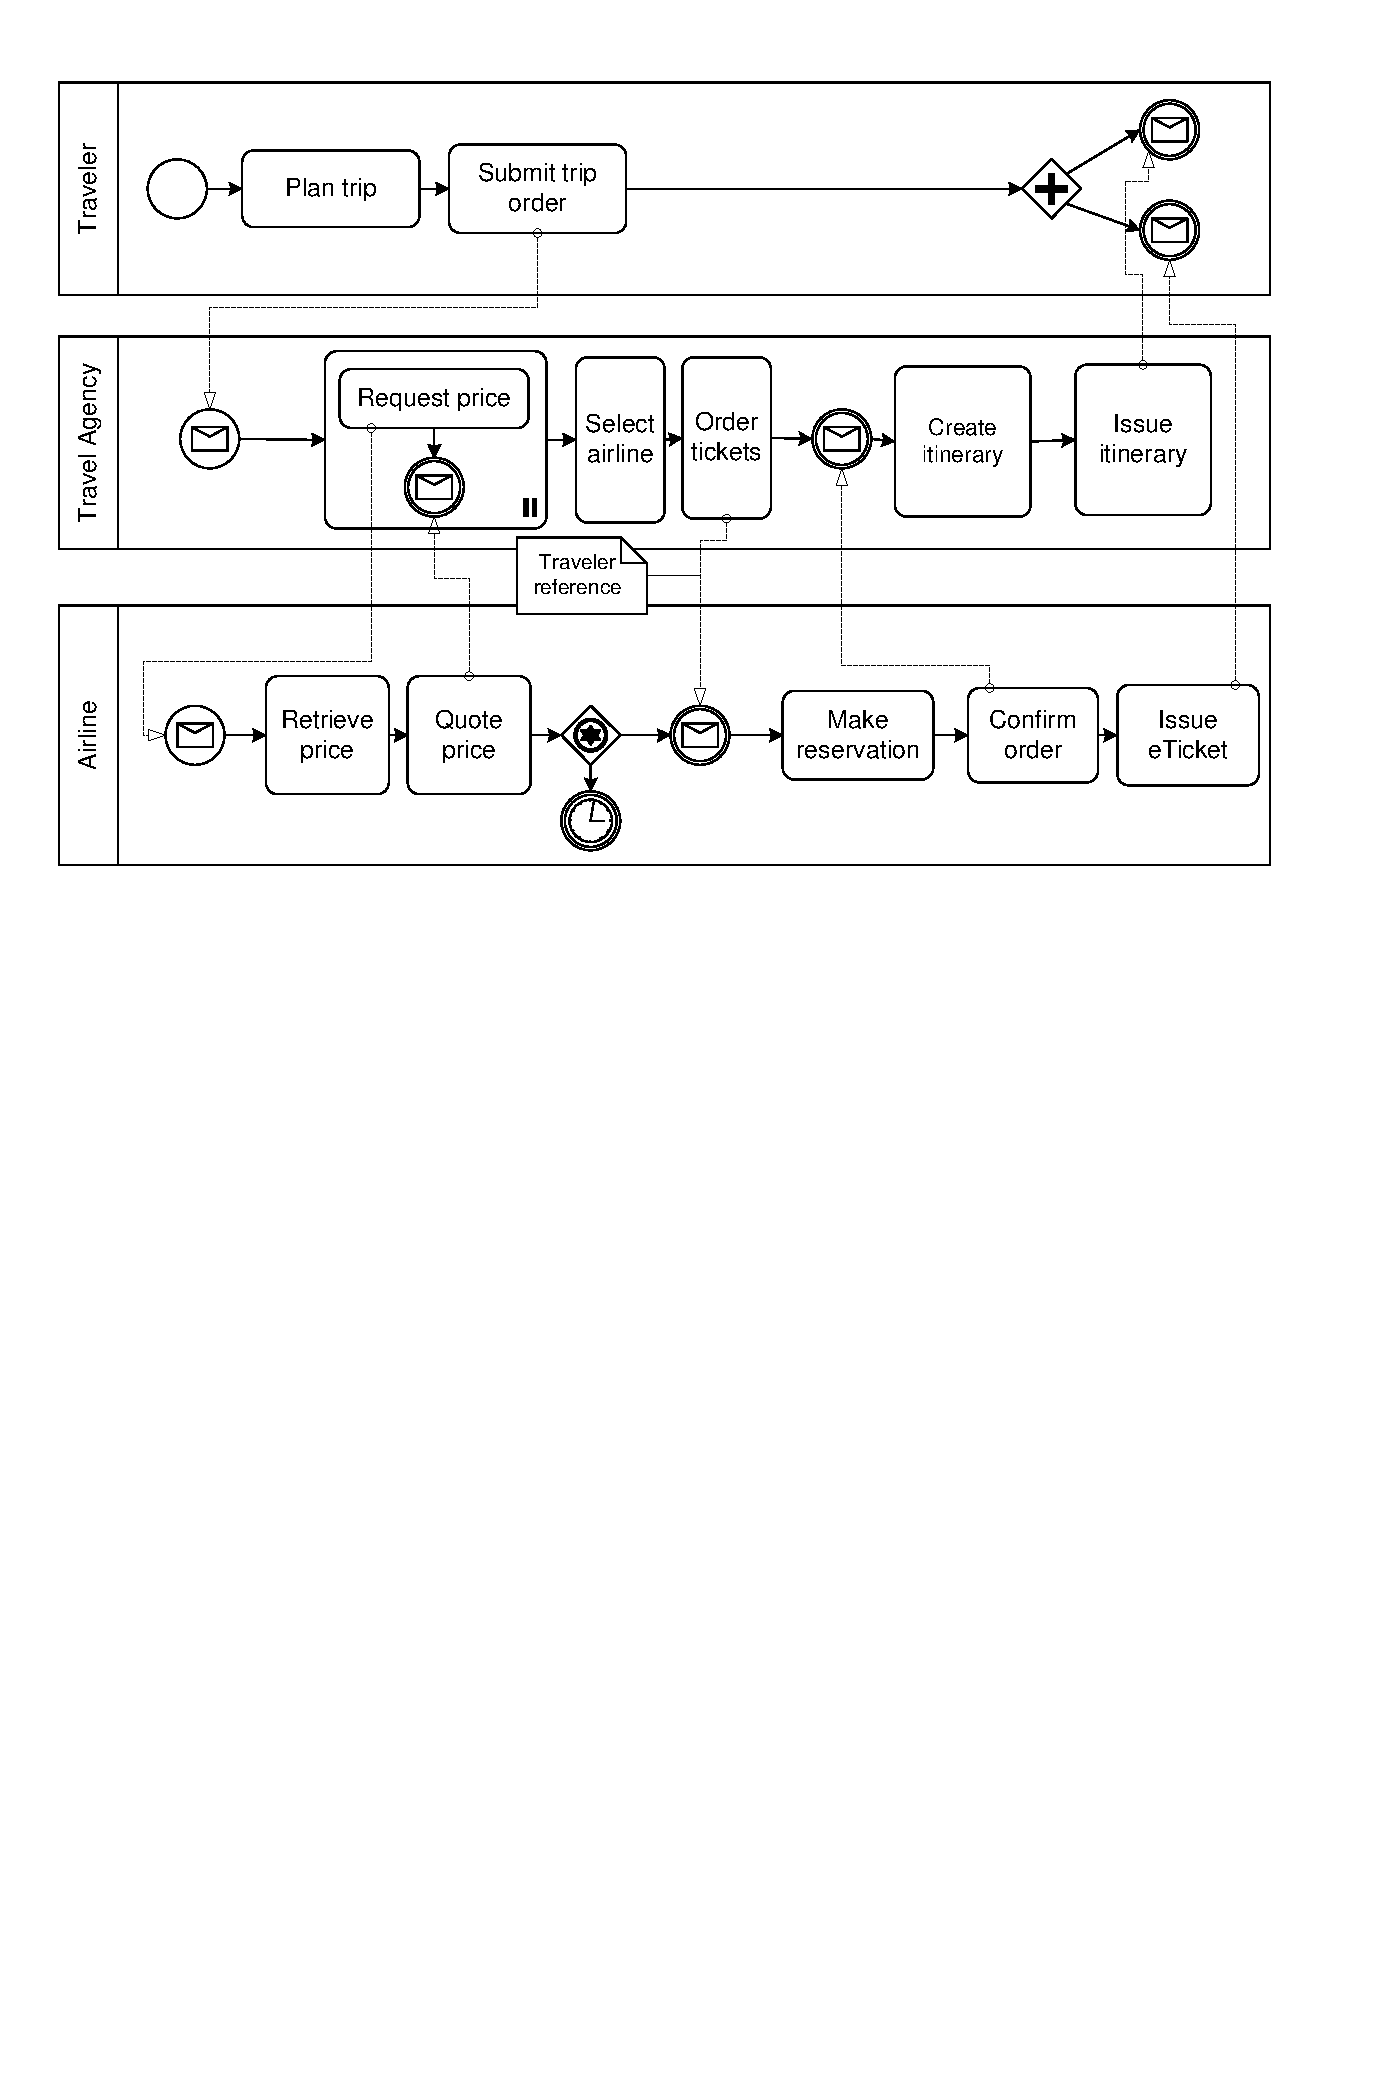
\includegraphics[width=\textwidth]{choreography}
    \caption{Beispiel-Choreographie}
    \label{fig:chor1}
  \end{center}
\end{figure}

\begin{figure}
  \begin{center}
    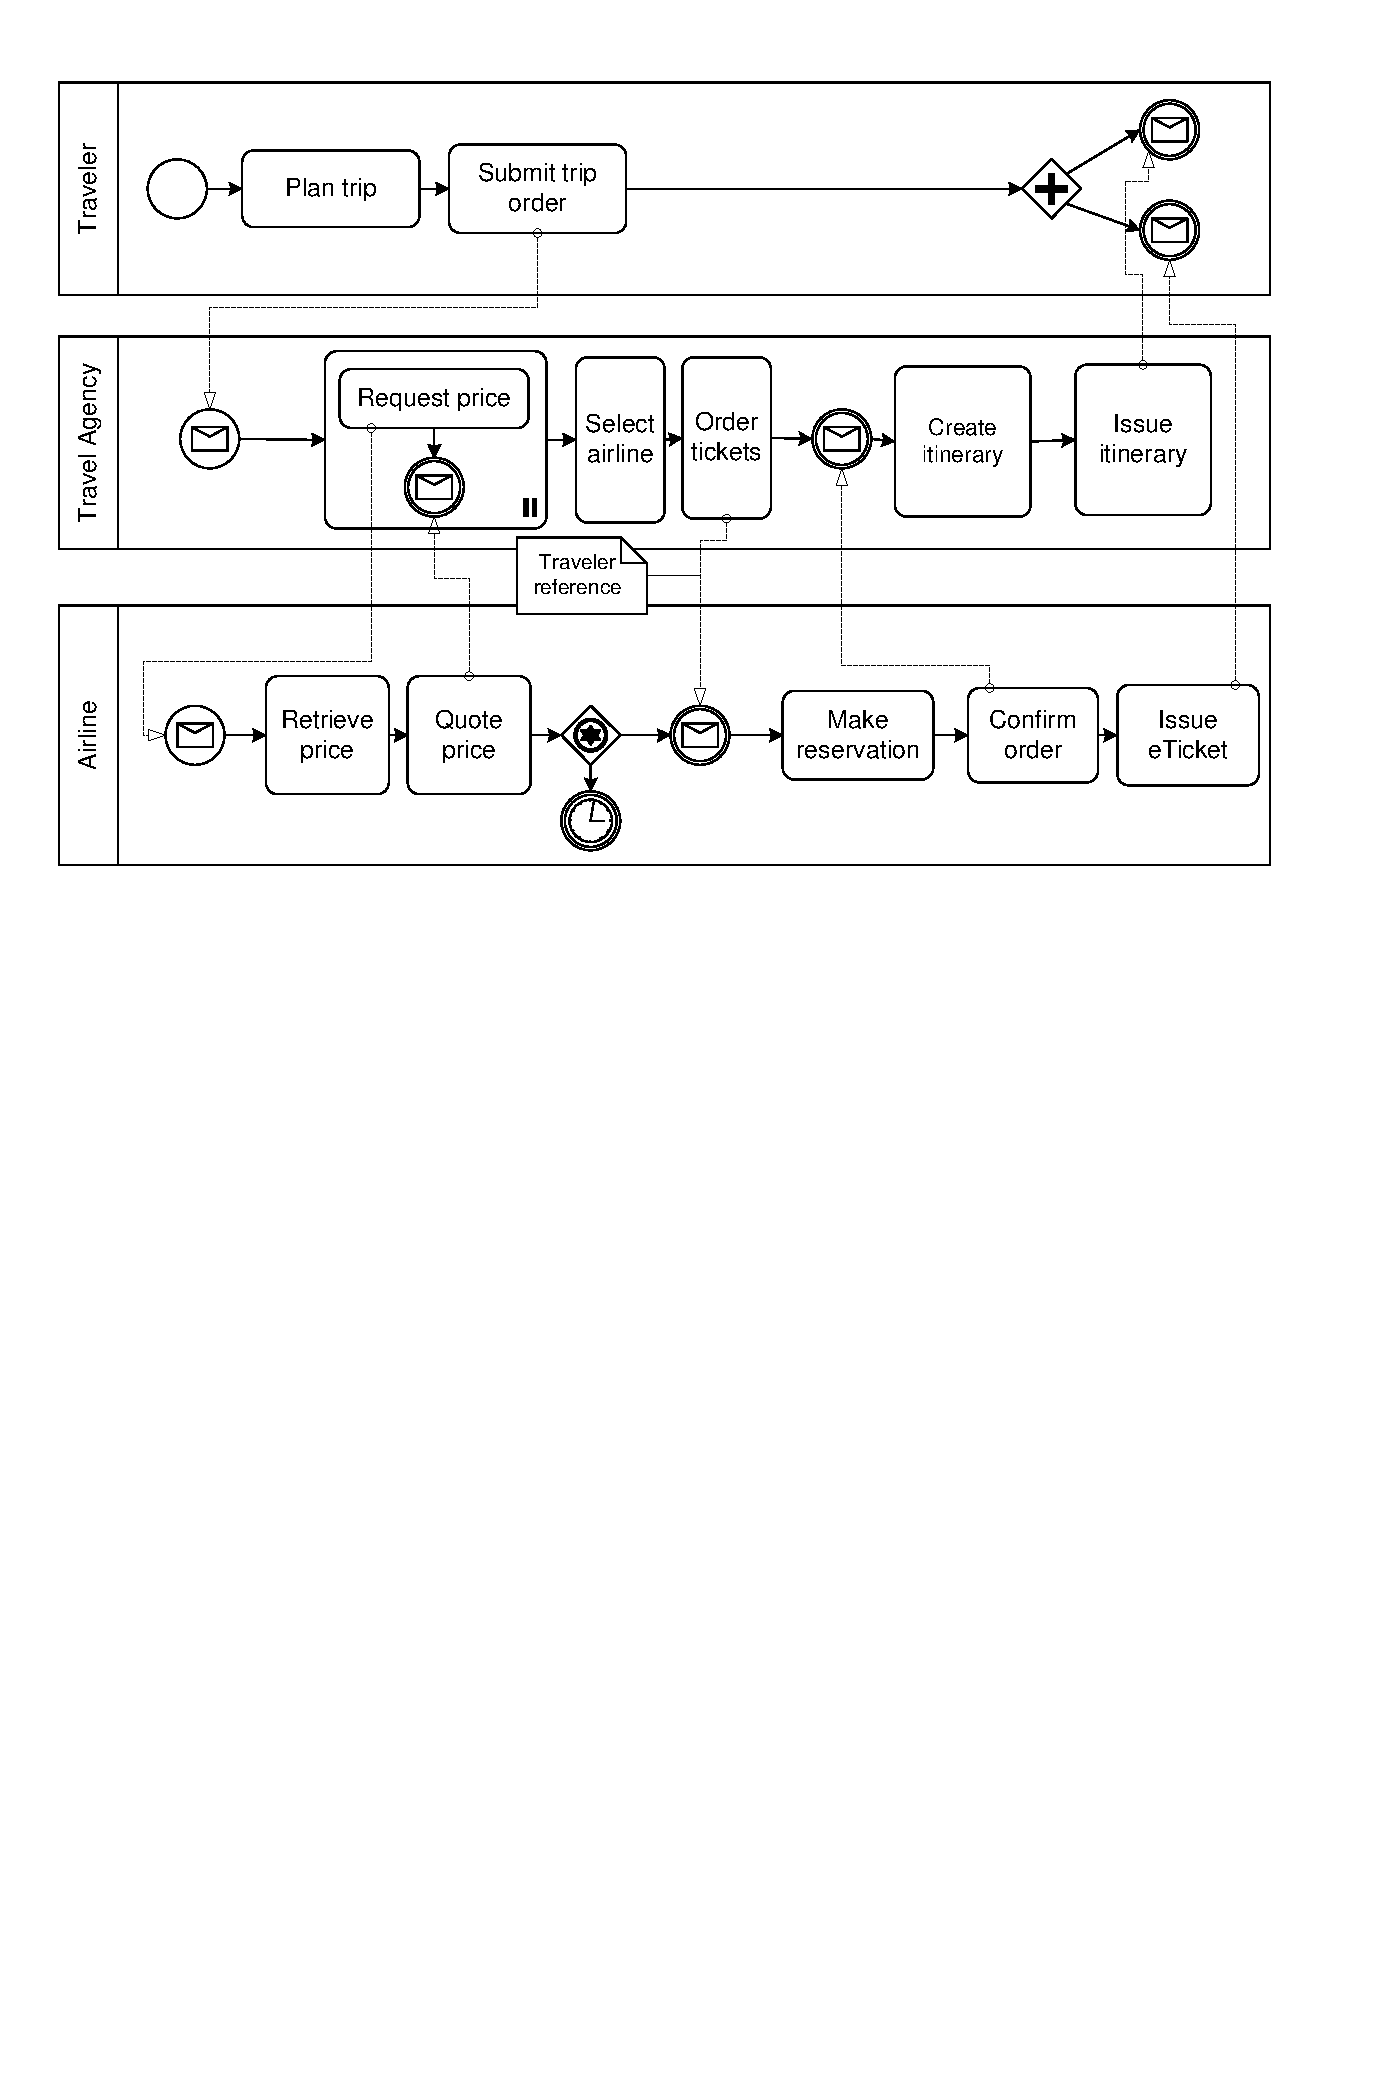
\includegraphics[width=.8\textwidth]{choreography}
    \caption[Beispiel-Choreographie]{Die Beispiel-Choreographie. Nun etwas kleiner, damit \texttt{\textbackslash textwidth} demonstriert wird. Und auch die Verwendung von alternativen Bildunterschriften für das Verzeichnis der Abbildungen. Letzteres ist allerdings nur Bedingt zu empfehlen, denn wer liesst schon so viel Text unter einem Bild? Oder ist es einfach nur Stilsache?}
    \label{fig:chor2}
  \end{center}
\end{figure}

\section{Tabellen}
Tabelle~\ref{tab:Ergebnisse} zeigt Ergebnisse.
\begin{table}
  \begin{center}
    \begin{tabular}{ccc}
	\toprule
	\multicolumn{2}{c}{\textbf{zusammengefasst}} & \textbf{Titel} \\ \midrule
	Tabelle & wie & in \\
	\url{tabsatz.pdf}& empfohlen & gesetzt\\
	
	\multirow{2}{*}{Beispiel} & \multicolumn{2}{c}{ein schönes Beispiel}\\
	 & \multicolumn{2}{c}{für die Verwendung von \gq{multirow}}\\
	\bottomrule
    \end{tabular}
    \caption[Beispieltabelle]{Beispieltabelle -- siehe \url{http://www.ctan.org/tex-archive/info/german/tabsatz/}}
    \label{tab:Ergebnisse}
  \end{center}
\end{table}

\section{Pseudocode}
Algorithmus~\vref{alg:sample} zeigt einen Beispielalgorithmus.
\begin{Algorithmus} %Die Umgebung nur benutzen, wenn man den Algorithmus ähnlich wie Graphiken von TeX platzieren lassen möchte
\caption{Sample algorithm}
\label{alg:sample}
\begin{algorithmic}
\Procedure{Sample}{$a$,$v_e$}
\State $\mathsf{parentHandled} \gets (a = \mathsf{process}) \lor \mathsf{visited}(a'), (a',c,a) \in \mathsf{HR}$ 
\State \Comment $(a',c'a) \in \mathsf{HR}$ denotes that $a'$ is the parent of $a$
\If{$\mathsf{parentHandled}\,\land(\mathcal{L}_\mathit{in}(a)=\emptyset\,\lor\,\forall l \in \mathcal{L}_\mathit{in}(a): \mathsf{visited}(l))$}
\State $\mathsf{visited}(a) \gets \text{true}$
\State $\mathsf{writes}_\circ(a,v_e) \gets
\begin{cases}
\mathsf{joinLinks}(a,v_e) & \abs{\mathcal{L}_\mathit{in}(a)} > 0\\
\mathsf{writes}_\circ(p,v_e)
& \exists p: (p,c,a) \in \mathsf{HR}\\
(\emptyset, \emptyset, \emptyset, false) & \text{otherwise}
\end{cases}
$
\If{$a\in\mathcal{A}_\mathit{basic}$}
  \State \Call{HandleBasicActivity}{$a$,$v_e$}
\ElsIf{$a\in\mathcal{A}_\mathit{flow}$}
  \State \Call{HandleFlow}{$a$,$v_e$}
\ElsIf{$a = \mathsf{process}$} \Comment Directly handle the contained activity
  \State \Call{HandleActivity}{$a'$,$v_e$}, $(a,\bot,a') \in \mathsf{HR}$
  \State $\mathsf{writes}_\bullet(a) \gets \mathsf{writes}_\bullet(a')$
\EndIf
\ForAll{$l \in \mathcal{L}_\mathit{out}(a)$}
  \State \Call{HandleLink}{$l$,$v_e$}
\EndFor
\EndIf
\EndProcedure
\end{algorithmic}
\end{Algorithmus}

\clearpage
Und wer einen Algorithmus schreiben möchte, der über mehrere Seiten geht, der kann das nur mit folgendem \textbf{üblen} Hack tun:

{
\begin{minipage}{\textwidth}
\hrule height .8pt width\textwidth
\vskip.15em%\vskip\abovecaptionskip\relax
\stepcounter{Algorithmus}
\addcontentsline{alg}{Algorithmus}{\protect\numberline{\theAlgorithmus}{\ignorespaces Description \relax}}
\noindent\textbf{Algorithmus \theAlgorithmus} Description
%\stepcounter{algorithm}
%\addcontentsline{alg}{Algorithmus}{\thealgorithm{}\hskip0em Description}
%\textbf{Algorithmus \thealgorithm} Description
\vskip.3em%\vskip\belowcaptionskip\relax
\hrule height .5pt width\textwidth
\end{minipage}
code goes here\\
test2\\
\vskip-.9em
\hrule height .5pt width\textwidth
}

\section{Verschiedenes}
\label{sec:diff}
Ziffern (123\,654\,789) werden schön gesetzt. Falls dies nicht gewünscht ist, den Parameter \texttt{osf} bei dem Paket \texttt{mathpazo} herausnehmen.

\textsc{Kapitälchen} werden schön gesperrt...

\begin{compactenum}[I]
\item Man kann auch die Nummerierung dank paralist kompakt halten
\item und auf eine andere Nummerierung umstellen
\end{compactenum}

\section{Weitere Hinweise}
Bitte schaut für weitere Informationen in's Studiwiki\footnote{\url{http://studiwiki.informatik.uni-stuttgart.de/LaTeX}}. Dort sind viele weitere Tipps und Hinweise verlinkt.

Verbesserungsvorschläge für diese Vorlage sind immer willkommen. Bitte im Trac ein Ticket eingragen (\url{https://vorlagen.studiforge.informatik.uni-stuttgart.de/trac.fcgi/wiki/WikiStart}).

\chapter{Zusammenfassung und Ausblick}\label{chap:zusfas}
Hier bitte einen kurzen Durchgang durch die Arbeit.

\section*{Ausblick}
...und anschließend einen Ausblick


%
%
%\renewcommand{\appendixtocname}{Anhang}
%\renewcommand{\appendixname}{Anhang}
%\renewcommand{\appendixpagename}{Anhang}
\appendix
\chapter{Ein Anhang}
...falls gewünscht...

Und hier noch ein Text aus dem Projekt Gutenberg zum Test der Ränder und des optischen Randausgleichs

Des Lebens Überfluss\footnote{\url{http://gutenberg.spiegel.de/tieck/ueberflu/ueberflu.htm}} von Ludwig Tieck.

In einem der härtesten Winter war gegen Ende des Februar ein sonderbarer Tumult gewesen, über dessen Entstehung, Fortgang und Beruhigung die seltsamsten und widersprechendsten Gerüchte in der Residenz umliefen. Es ist natürlich, dass, wenn alle Menschen sprechen und erzählen wollen, ohne den Gegenstand ihrer Darstellung zu kennen, auch das Gewöhnliche die Farbe der Fabel annimmt.

In der Vorstadt, die ziemlich bevölkert ist hatte sich in einer der engsten Straßen das Abenteuer zugetragen. Bald hieß es, ein Verräter und Rebell sei entdeckt und von der Polizei aufgehoben worden, bald, ein Gottesleugner, der mit andern Atheisten verbrüdert das Christentum mit seiner Wurzel ausrotten wollen, habe sich nach hartnäckigem Widerstand den Behörden ergeben und sitze nun so lange fest, bis er in der Einsamkeit bessere Grundsätze und Überzeugungen finde. Er habe sich aber vorher noch in seiner Wohnung mit alten Doppelhaken, ja sogar mit einer Kanone verteidigt, und es sei, bevor er sich ergeben, Blut geflossen, so dass das Konsistorium wie das Kriminalgericht wohl auf seine Hinrichtung antragen werde. Ein politischer Schuhmacher wollte wissen, der Verhaftete sei ein Emissär, der als das Haupt vieler geheimen Gesellschaften mit allen Revolutionsmännern Europas in innigster Verbindung stehe; er habe alle Fäden in Paris, London und Spanien wie in den östlichen Provinzen gelenkt, und es sei nahe daran, dass im äußersten Indien eine ungeheure Empörung ausbrechen und sich dann gleich Cholera nach Europa herüberwälzen werde, um allen Brennstoff in lichte Flammen zu setzen.

So viel war ausgemacht, in einem kleinen Hause hatte es Tumult gegeben, die Polizei war herbeigerufen worden, das Volk hatte gelärmt, angesehene Männer wurden bemerkt, die sich darein mischten, und nach einiger zeit war alles wieder ruhig, ohne dass man den Zusammenhang begriff. Im Hause selbst war eine gewisse Zerstörung nicht zu verkennen. Jeder legte sich die Sache aus, wie Laune oder Phantasie sie ihm erklären mochten. Die Zimmerleute und Tischler besserten nachher den Schaden aus.

Ein Mann hatte in diesem Hause gewohnt, den niemand in der Nachbarschaft kannte. War er ein Gelehrter? ein Politiker? ein Einheimischer? ein Fremder? Darüber wusste keiner, selbst der Klügste nicht, einen genügenden Bescheid zu geben.

Soviel ist gewiss, dieser unbekannte Mann lebte sehr still und eingezogen, man sah ihn auf keinem Spaziergange, an keinem öffentlichen Orte. Er war noch nicht alt, wohlgebildet, und seine junge Frau, die sich mit ihm dieser Einsamkeit ergeben hatte, durfte man eine Schönheit nennen.

Um Weihnachten war es, als dieser jugendliche Mann in seinem Stübchen, dicht am Ofen sitzend, also zu seiner Frau redete: »Du weißt, liebste Klara, wie sehr ich den Siebenkäs unsers Jean Paul liebe und verehre; wie dieser sein Humorist sich aber helfen würde, wenn er in unsrer Lage wäre, bleibt mir doch ein Rätsel. Nicht wahr, Liebchen, jetzt sind, so scheint es, alle Mittel erschöpft?«

»Gewiss, Heinrich«, antwortete sie lächelnd und zugleich seufzend; »wenn du aber froh und heiter bleibst, liebster aller Menschen, so kann ich mich in deiner Nähe nicht unglücklich fühlen.«

»Unglück und Glück sind nur leere Worte«, antwortete Heinrich; »als du mir aus dem Hause deiner Eltern folgtest, als du so großmütig um meinetwillen alle Rücksichten fahren ließest: da war unser Schicksal auf unsre Lebenszeit bestimmt. Lieben und leben hieß nun unsre Losung; wie wir leben würden, durfte uns ganz gleichgültig sein. Und so möchte ich noch jetzt aus starkem Herzen fragen: Wer in ganz Europa ist wohl so glücklich, als ich mich mit vollem Recht aus der ganzen Kraft meines Gefühles nennen darf?«

»Wir entbehren fast alles«, sagte sie, »nur uns selbst nicht, und ich wusste ja, als ich den Bund mit dir schloss, dass du nicht reich warst; dir war es nicht unbekannt, dass ich aus meinem väterlichen Hause nichts mit mir nehmen konnte. So ist die Armut mit unsrer Liebe eins geworden, und dieses Stübchen, unser Gespräch, unser Anblicken und Schauen in des Geliebten Auge ist unser Leben.«

»Richtig!« rief Heinrich aus und sprang auf in seiner Freude, um die Schöne lebhaft zu umarmen; »wie gestört, ewig getrennt, einsam und zerstreut wären wir nun in jenem Schwarm der vornehmen Zirkel, wenn alles in seiner Ordnung vor sich gegangen wäre. Welch Blicken, Sprechen, Handgeben, Denken dort! Man könnte sich Tiere oder selbst Marionetten so abrichten und eindrechseln, dass sie eben die Komplimente machten und solche Redensarten von sich gäben. So sind wir, mein Schatz, wie Adam und Eva hier in unserm Paradiese, und kein Engel kommt auf den ganz überflüssigen Einfall, uns daraus zu vertreiben.«

»Nur«, sagte sie etwas kleinlaut, »fängt das Holz an, ganz einzugehen, und dieser Winter ist der härteste, den ich bis jetzt noch erlebt habe.«

Heinrich lachte. »Sieh«, rief er, »ich muss aus purer Bosheit lachen, aber es ist darum noch nicht das Lachen der Verzweiflung, sondern einer gewissen Verlegenheit, da ich durchaus nicht weiß, wo ich Geld hernehmen könnte. Aber finden müssen sich die Mittel; denn es ist undenkbar, dass wir erfrieren sollten, bei so heißer Liebe, bei so warmem Blut! Pur unmöglich!«

Sie lachte ihn freundlich an und erwiderte: »Wenn ich nur so wie Lenette Kleider zum Verkaufe mitgebracht, oder überflüssige Messingkannen und Mörser oder kupferne Kessel in unsrer kleinen Wirtschaft umherständen, so wäre leicht Rat zu finden.«

»Jawohl«, sprach er mit übermütigem Ton, »wenn wir Millionärs wären, wie jener Siebenkäs, dann wäre es keine Kunst, Holz anzuschaffen und selbst bessere Nahrung.«

Sie sah im Ofen nach, in welchem Brot in Wasser kochte, um so das kärglichste Mittagsmahl herzustellen, welches dann mit einem Nachtisch von weniger Butter beschlossen werden sollte. »Während du«, sagte Heinrich, »die Aufsicht über unsre Küche führst und dem Koch die nötigen Befehle erteilst, werde ich mich zu meinen Studien niedersetzen. Wie gern schriebe ich wieder, wenn mir nicht Tinte, Papier und Feder völlig ausgegangen wären; ich möchte auch wieder einmal etwas lesen, was es auch sei, wenn ich nur noch ein Buch hätte.«

»Du musst denken, Liebster«, sagte Klara und sah schalkhaft zu ihm hinüber; »die Gedanken sind dir hoffentlich noch nicht ausgegangen.«

»Liebste Ehefrau«, erwiderte er, »unsre Wirtschaft ist so weitläuftig und groß, dass sie wohl deine ganze Aufmerksamkeit in Anspruch nimmt; zerstreue dich ja nicht, damit nicht unsre ökonomischen Verhältnisse in Verwirrung geraten. Und da ich mich jetzt in meine Bibliothek begebe, so lass mich vor jetzt in Ruhe; denn ich muss meine Kenntnisse erweitern und meinem Geiste Nahrung gönnen.«

»Er ist einzig!« sagte die Frau zu sich selber und lachte fröhlich; »und wie schön er ist!«

»So lese ich denn wieder in meinem Tagebuche«, sprach Heinrich, »das ich ehemals anlegte, und es interessiert mich, rückwärts zu studieren, mit dem Ende anzufangen und mich so nach und nach zu dem Anfange vorzubereiten, damit ich diesen um so besser verstehe. Immer muss alles echte Wissen, alles Kunstwerk und gründliche Denken in einen Kreis zusammenschlagen und Anfang und Ende innigst vereinigen, wie die Schlange, die sich in den Schwanz beißt – ein Sinnbild der Ewigkeit, wie andre sagen; ein Symbol des Verstandes und alles Richtigen, wie ich behaupte.«

Er las auf der letzten Seite, aber nur halblaut: »Man hat ein Märchen, dass ein wütender Verbrecher, zum Hungertode verdammt, sich selber nach und nach aufspeiset; im Grunde ist das nur die Fabel des Lebens und eines jeden Menschen. Dort blieb am Ende nur der Magen und das Gebiss übrig, bei uns bleibt die Seele, wie sie das Unbegreifliche nennen. Ich aber habe mich abgestreift und abgelebt. Es war beinah lächerlich, dass ich noch einen Frack nebst Zubehör besaß, da ich niemals ausgehe. Am Geburtstage meiner Frau werde ich in Weste und Hemdärmeln vor ihr erscheinen, da es doch unschicklich wäre, bei hoffährigen Leuten in einem ziemlich abgetragenen Überrock Cour zu machen.«

»Hier geht die Seite und das Buch zu Ende«, sagte Heinrich. »Alle Welt sieht ein, dass unsre Fracks eine dumme und geschmacklose Kleidung sind, alle schelten diese Uniform, aber keiner macht, so wie ich, Ernst damit, den Plunder ganz abzuschaffen. Ich erfahre nun nicht einmal aus den Zeitungen, ob andere Denkende meinem kühnen Beispiele und Vorgange folgen werden.«

Er schlug um und las die vorige Seite: »Man kann auch ohne Servietten leben. Wenn ich bedenke, wie unsre Lebensweise immer mehr und mehr in Surrogat, Stellvertretung und Lückenbüßerei übergegangen ist, so bekomme ich einen rechten Hass auf unser geiziges und knickerndes Jahrhundert und fasse, da ich es ja haben kann, den Entschluss, in der Weise unsrer viel freigebigern Altvordern zu leben. Diese elenden Servietten sind ja, was selbst die heutigen Engländer noch wissen und verachten, offenbar nur erfunden, um das Tischtuch zu schonen. Ist es also Großmut, das Tischtuch nicht zu achten, so gehe ich darin noch weiter, das Tafeltuch zusamt den Servietten für überflüssig zu erklären. Beides wird verkauft, um vom saubern Tische selbst zu essen, nach Weise er Patriarchen, nach Art der – nun? welcher Völker? Gleichviel! Essen doch viele Menschen selbst ohne Tisch. Und, wie gesagt, ich treibe dergleichen nicht aus zynischer Sparsamkeit, nach Art des Diogenes, aus dem Hause, sondern im Gegenteil im Gefühl meines Wohlstandes, um nur nicht, wie die jetzige Zeit, aus törichtem Sparen zum Verschwender zu werden.«

»Du hast es getroffen«, sagte die Gattin lächeln; »aber damals lebten wir von dem Erlös dieser überflüssigen Sachen doch noch verschwenderisch. Oft sogar hatten wir zwei Schüsseln.«

Jetzt setzten sich die beiden Gatten zum dürftigsten Mahle nieder. Wer sie gesehen, hätte sie für beneidenswerte halten müssen, so fröhlich, ja ausgelassen waren sie an der einfachen Tafel. Als die Brotsuppe verzehrt war holte Klara mit schalkhafter Miene einen verdeckten Teller aus dem Ofen und setzte dem überraschten Gatten noch einige Kartoffeln vor. »Sieh!« rief dieser, »das heißt einem, wenn man sich an den vielen Büchern satt studiert hat, eine heimliche Freude machen! Dieser gute Erdapfel hat mit zu der großen Umwälzung von Europa beigetragen. Der Held Walter Raleigh soll leben!« – Sie stießen mit den Wassergläsern an, und Heinrich sah nach, ob der Enthusiasmus auch nicht einen Riss im Glase verursacht habe. »Um diese ungeheure Künstlichkeit«, sagte er dann, »um diese Einrichtung mit unsern alltäglichen Gläsern würden uns die reichsten Fürsten des Altertums beneidet haben. Es muss langweilig sein, aus einem goldenen Pokal zu trinken, vollends so schönes, klares, gesundes Wasser. Aber in unsern Gläsern schwebt die erfrischende Welle so heiter durchsichtig, so eins mit dem Becher, dass man wirklich versucht wird, zu glauben, man genieße den flüssig gewordenen Äther selbst. – Unsre Mahlzeit ist geschlossen; umarmen wir uns.«

\section{Weitere Illustrationen}
Abbildungen~\ref{fig:AnhangsChor} und~\ref{fig:AnhangsChor2} zeigen zwei Choreographien, die den
Sachverhalt weiter erläutern sollen. Die zweite Abbildung ist um 90 Grad gedreht, um das Paket
\texttt{rotating} zu demonstrieren.

\begin{figure}
  \begin{center}
    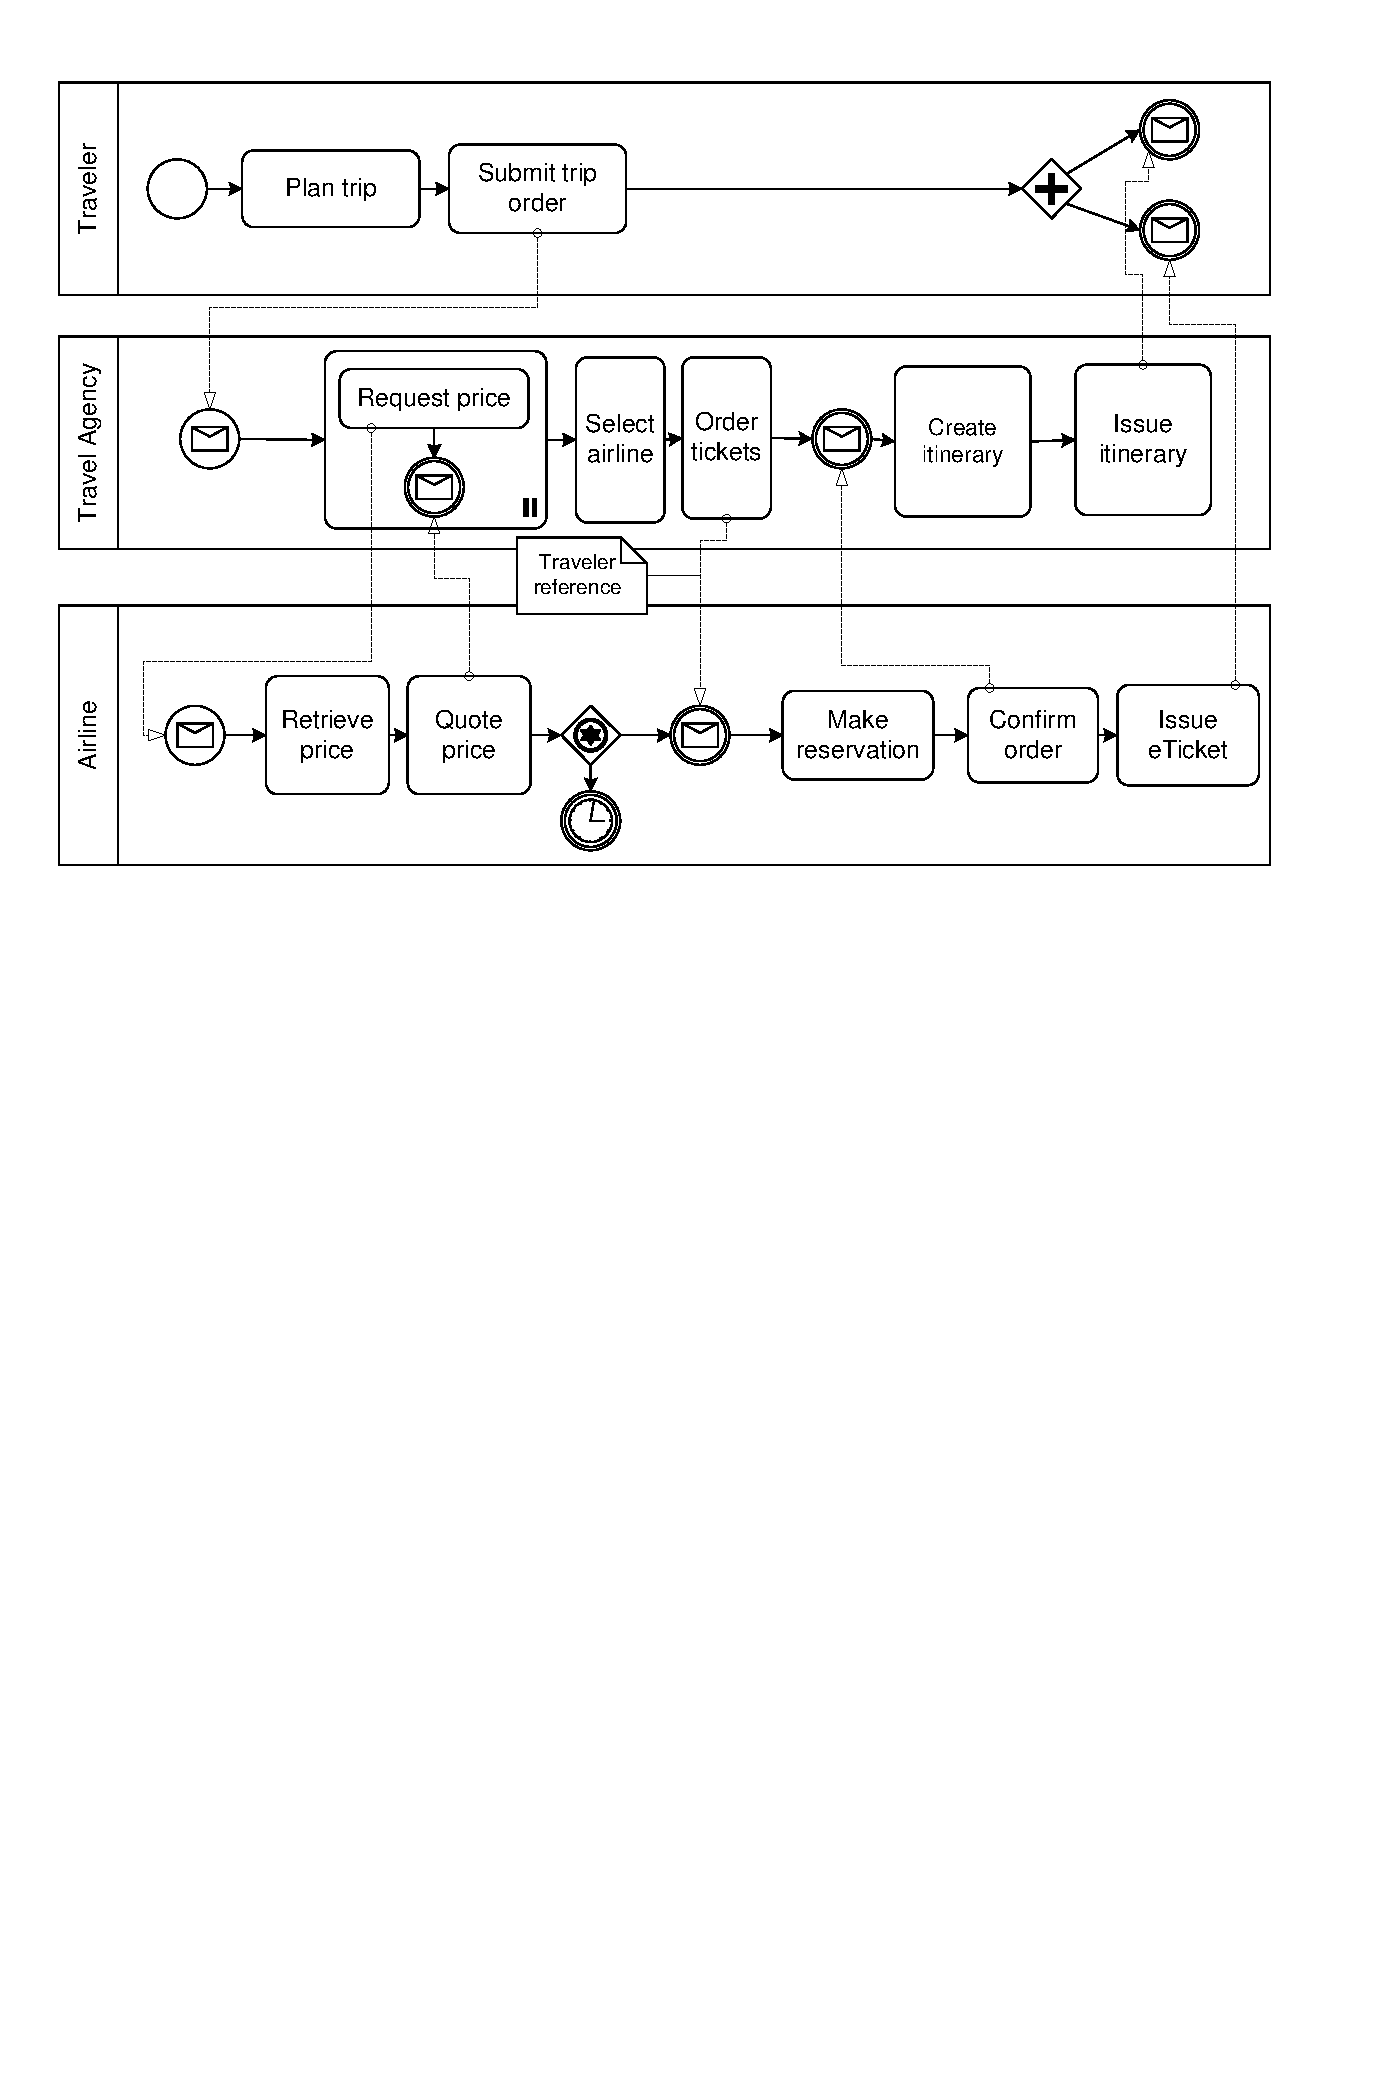
\includegraphics[width=\textwidth]{choreography.pdf}
    \caption{Beispiel-Choreographie I}
    \label{fig:AnhangsChor}
  \end{center}
\end{figure}

\begin{landscape}
%sidewaysfigure
\begin{figure}
  \begin{center}
    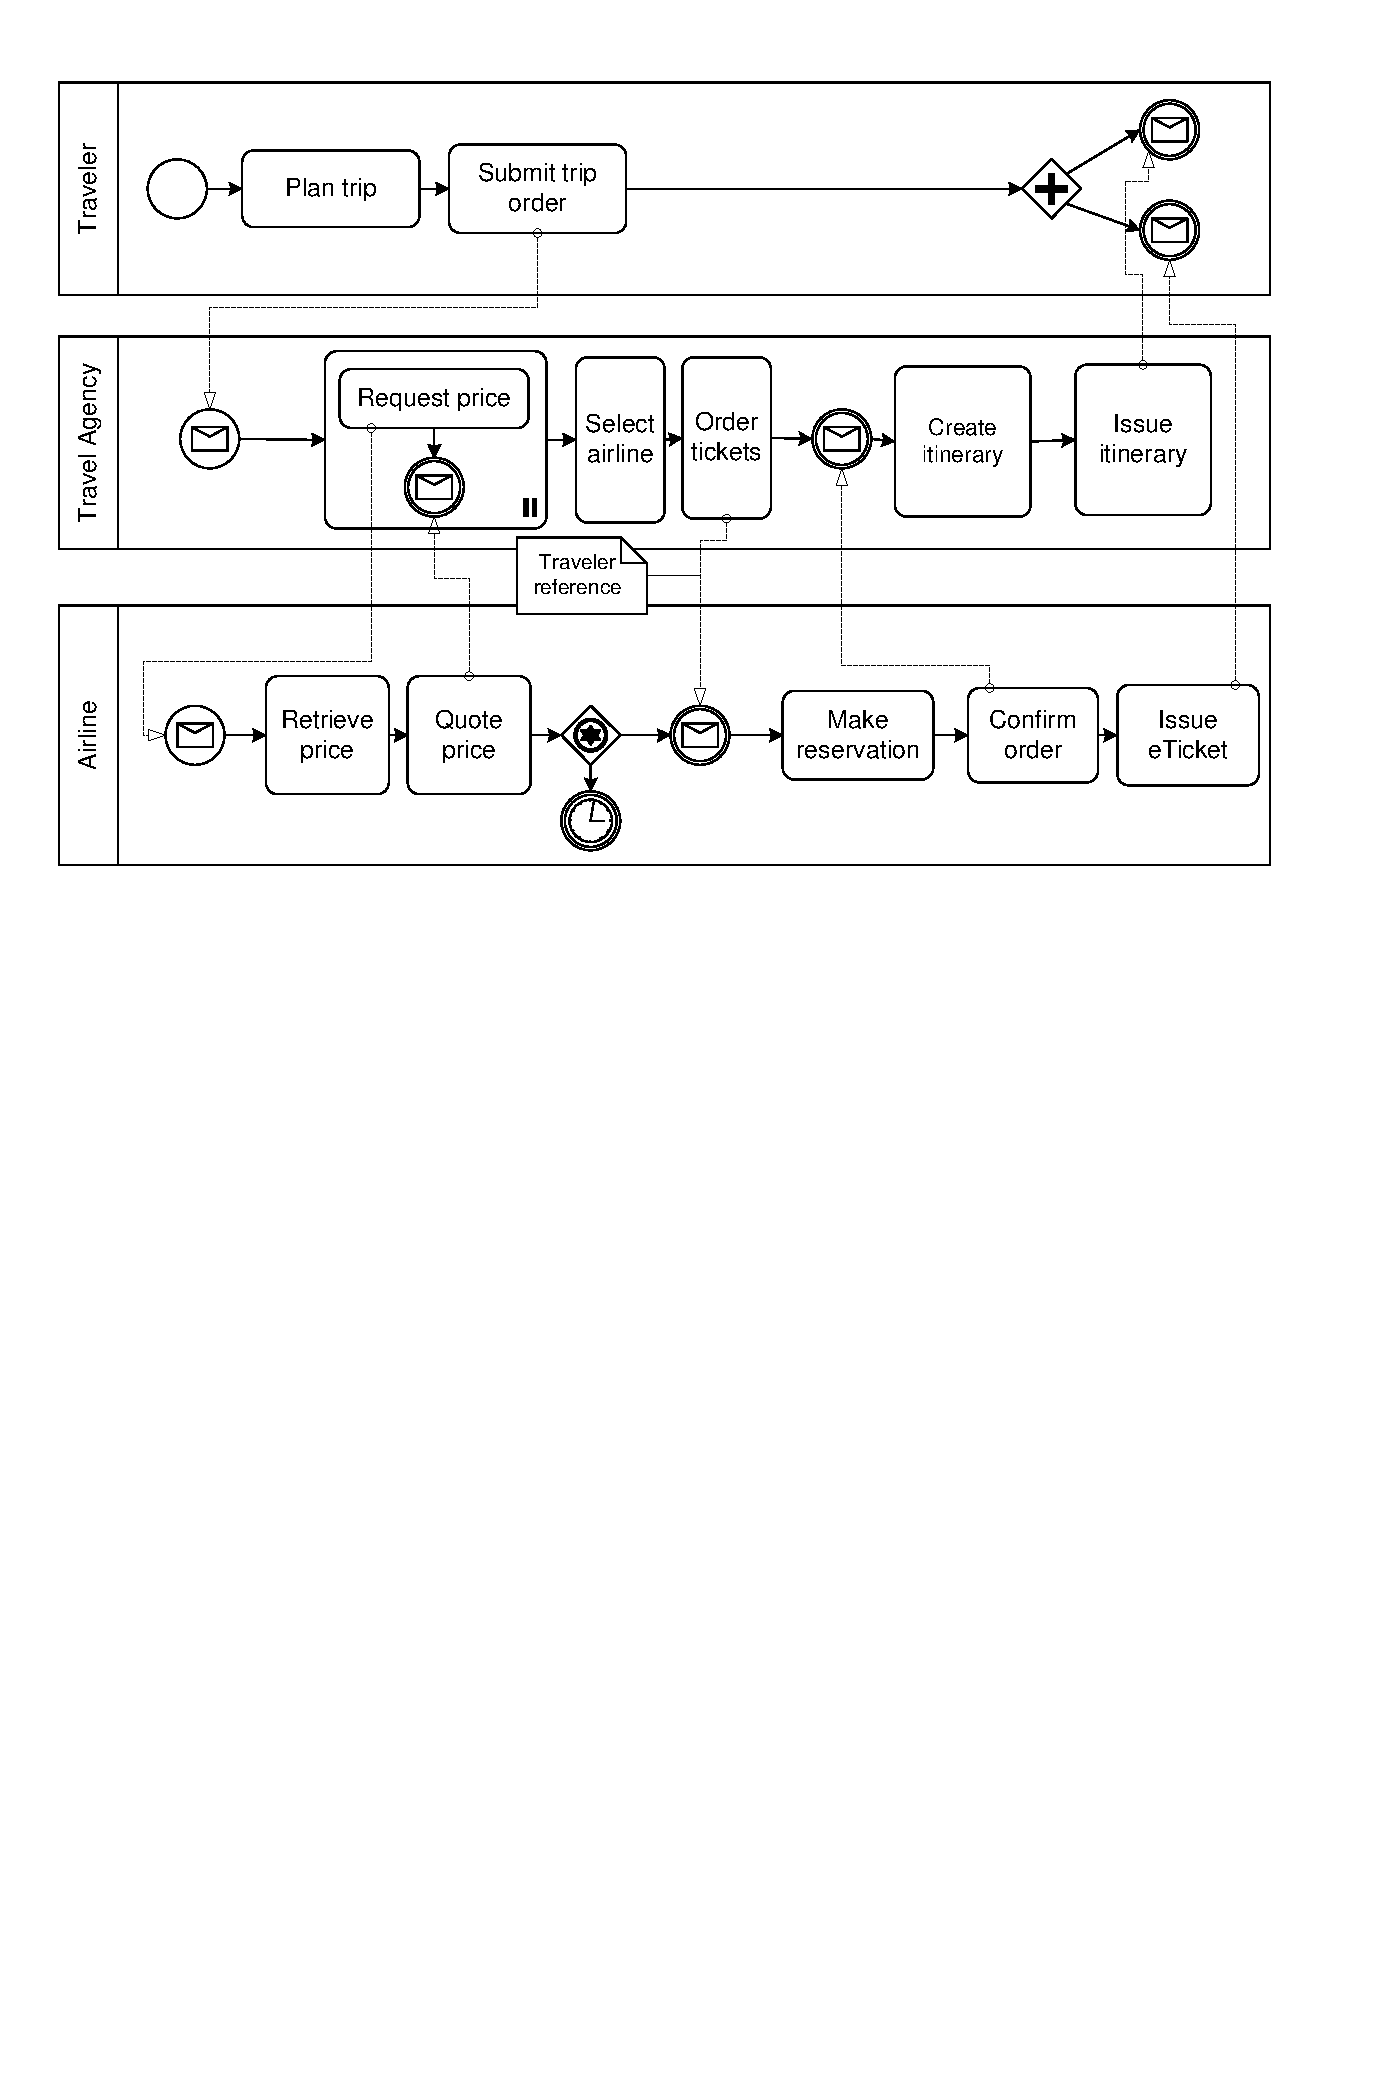
\includegraphics[width=\textwidth]{choreography.pdf}
    \caption{Beispiel-Choreographie II}
    \label{fig:AnhangsChor2}
  \end{center}
\end{figure}
\end{landscape}

%\printindex
%\bibliographystyle{alphadin}
\ifdeutsch
\bibliographystyle{bibliography/IAASde} %f"ur deutsche Texte
\else
\bibliographystyle{bibliography/IAAS} %f"ur englische Texte
\fi
\bibliography{bibliography/bibliography}
\ifdeutsch
Alle URLs wurden zuletzt am 17.03.2008 gepr\"uft.
\else
All links were last followed on March 17, 2008.
\fi

\backmatter 
\pagestyle{empty}
\renewcommand*{\chapterpagestyle}{empty}
\Versicherung
\end{document}
